\documentclass[12pt]{article}
\def\x#1#2{$\mathbb{#1}^#2$} 
\def\n#1{\x#1}

\usepackage{graphicx}
\usepackage{latexsym}
\usepackage{amsfonts}
\usepackage{amsmath}
\usepackage{listings}
\usepackage{mypriptrt}
\usepackage{subfigure}
\usepackage{epic}


\title{NC LU - Abgabe 2} 
\author{Kern, Weichselbaum}

\abstract{
	Documentation for the first exercise of Neural Computation LU, Group 8.
}
\begin{document}
	
	
\maketitle	

\section{Einführung}

% Die abgegebenen Dateien sind: calc_bias.m, calculate_weights.m, circle.m, draw_plot.m, draw_plot_rbf.m, genData.m, genDataRbf.m, generate_random_data.m, paintTraining.m, predictSVM.m, predictSVMRbf.m, predictSVMRbfws.m, rbfkernel.m, run.m, run_rbf.m, trainSVM.m, trainSVMRbf.m.
% \\
% \\
% Zum Laufen wird das Ganze durch run.m gebracht. Diese Funktion hat keine Parameter und exekutiert den Code fuer 2.1, 2.2 und 2.3.

\section{SVM, Aufgabe 2}

Die Daten erzeugen wir mit derselben Funktion wie bei Aufgabe 1. Dies wird ueber ie Std. Abweichung und Durchschnitt geregelt.
\\
Die $alpha$ werden mit Matlab's quadprog erzeugt. Diese quadprog Funktion wird gefuettert mit der Lagrange-Funktion in Matrix-Form $-0.5 \boldsymbol{\alpha}^T\mathbf{H}\boldsymbol{\alpha} + \mathbf{f}^T\boldsymbol{\alpha}$. $H$ in unserem Fall ist $H_{ij} = y_iy_j(\mathbf{x}_i\mathbf{x}_j)$ und $f$ ist der Einheitsvektor $f = \mathbf{1} = [1 ... 1 ... 1]^T$. Als Constraints verwenden wir $\alpha > 0$ und $y^T\alpha = 0$.
\\
\\
Da wir den Gewichtsvektor nicht augmentieren berechnen wir uns den Bias mit den Supportvektoren. Dies geschieht ueber 
\\
$\displaystyle b_0 = \frac{1}{N_{SV}} *  \sum_{s=1}^{N_{SV}} (\frac{1}{y_s} - \mathbf{x_s}^T\mathbf{w_0}) $, $s = 1, N_{SV}$
\\
und wird innerhalb der decision rule, welche wir in $predictSVM()$ implementiert haben, verwendet.
\\
\\
Laut Folien wird bei der decision rule das innere Produkt von $\mathbf{X}$ und $\mathbf{x_i}$ verwendet. Dies tun wir nicht und speichern den Gewichtsvektor direkt ab um nicht jedesmal zu summieren bzw. um den Code wiederverwrenden zu koennen.
\\
\\
Bei linear seperierbare Daten ist bei einer Crossvalidation von 80/20 eine 100\%ige Vorhersage des Klassenlabels gegeben.
\\
\\
Abbildung \ref{fig:lin} zeigt die 10 Datensaetze und die Hyperplane fuer die 10 geforderten linear seperierbaren Datensaetze.
\\
\begin{figure}[htp]
	\centering
	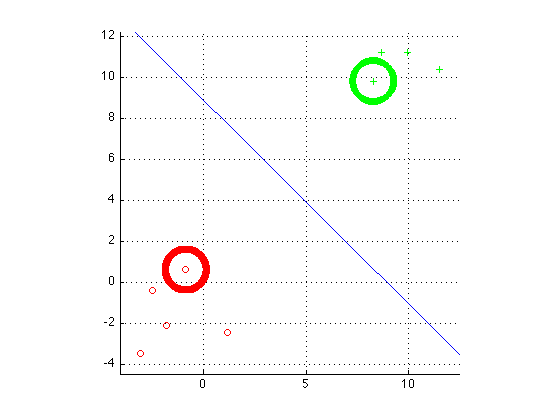
\includegraphics[width=1\textwidth]{linear_sep_data_plot}
	\caption{Datensatz, linear seperierbar, geplottet in Matlab. + ist Klasse 1, o signalisiert Klasse -1. Vektoren mit einem Kreis zeigen die Supportvektoren. Die Hyperplane ist optimal, da der Margin zwischen den Supportvektoren maximal ist.}
	\label{fig:lin}
\end{figure}
\\
Fuer \textbf{Beispiel 3} haben wir einige Daten kopiert und fuer den RBF-Kernel angepasst. Die Funktion $rbfkernel()$ wird mit dem regulaeren Kernel (dh. ein gausscher RBF-Kernel) implementiert und im umgeschriebenen $predictSVM$ verwendet.
\\
Anders als in Beispiel 2.2 wurde hier das innere Produkt verwendet und das $sigma$ als Parameter erweitert, so dass ein Test der Vorhersagefaehigkeit unserer SVM durchgefuehrt werden konnte.\\
Leider wurde dadurch die Faehigkeit verloren, den Gewichtsvektor im vorhinein zu berechnen und nur mehr mit der neuen Beobachtung zu multiplizieren. Allerdings hat diese Einschraenkung keinen Einfluss auf die Performance des Systems, da wir lediglich 100 2D-Teset-Datensaetze erzeugt haben.
\\
\\
Die Werte fuer $sigma$ haben keinen Einfluss auf die Entscheidung bei linear seperierbaren Daten, wenn sie so deutlich voneinander entfernt sind wie in unserem Fall. Erst wenn die Supportvektoren nahe der Hyperplane sind ist die Auswahl von $sigma$ entscheidend.
\\
Sigma stellt die Standardabweichung innerhalb der Klassen dar, welche wir erwarten. Liegen die beiden Klassen nun nah beieinander besteht die Möglichkeit, dass diese sich bei einer großen Standardabweichung überschneiden und Datensets nicht mehr eindeutig einer Klasse zuordenbar sind.
\\
Dies wurde probiert mit Werten von 0.1 bis 100 in 0.1 Schritten, keine neuen Beobachtungen wurden falsch vorhergesagt.
\\
\\
Bei den Schlupfvariablen haben wir die Lektuere von Kecman \cite{kecman} verwendet. Diese besagt, dass sich die Hesse-Notation der Lagrangen Funktion nicht veraendert. Lediglich die Constraints fuer $\boldsymbol{\alpha}$ aendert sich. Der Upperbound von $\boldsymbol{\alpha}$ ist nun nicht unendlich, sondern der Regulierungsparameter $C$.
\\
Dies ist insofern bedeutend, als das die Vektoren, welche nicht linear geteilt werden koennen, zu Supportvektoren der groesse $C$ gemacht werden.
\\
Abbildung \ref{fig:contour} zeigt die Vektoren in Hoehendarstellung und deren tatsaechlichen vorhergesagten Wert (dh. $predictSVM()$ ohne signum).

\begin{figure}[htp]
	\centering
	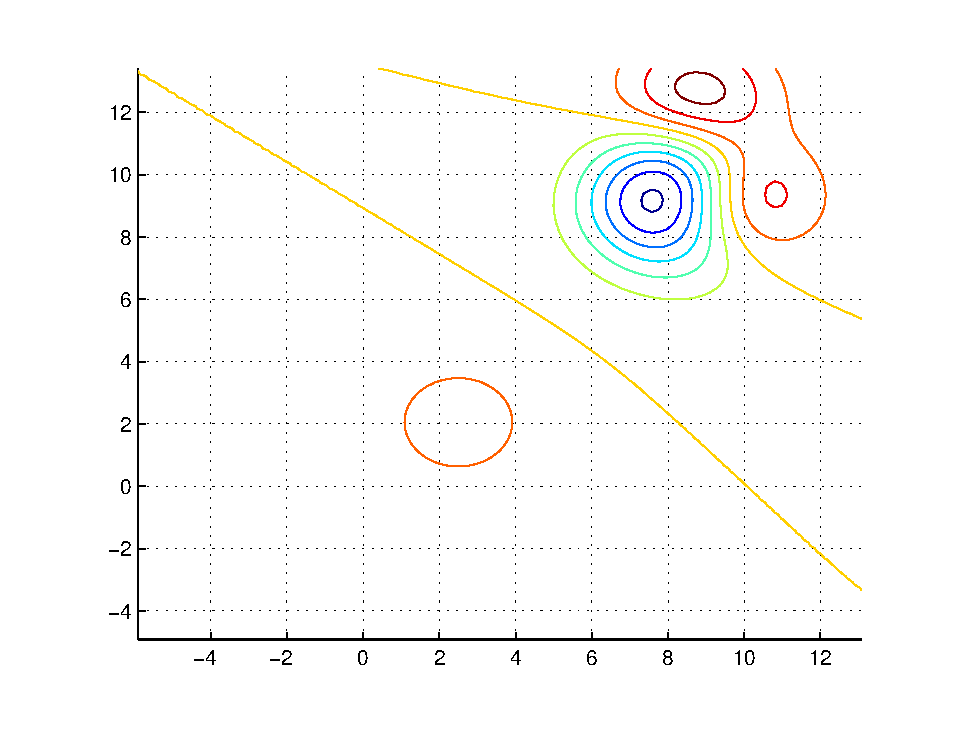
\includegraphics[width=1\textwidth]{contour}
	\caption{Datensatz, nicht linear seperierbar, mit contour in Matlab geplottet. Zeigt die Struktur des Datensatzes an Hand der gefunden Klassen.}
	\label{fig:contour}
\end{figure}

\bibliographystyle{plain}
\bibliography{docs}

\end{document}